\documentclass{article}
\usepackage[utf8]{inputenc}
\usepackage{xcolor}
\usepackage{textcomp}
\usepackage{graphicx}
\usepackage{amsthm}
\usepackage{macros}

\title{CIS 425 - Week 1 - Lecture 1}
\author{Alexander Eldemir}
\date{1 April 2019}

\begin{document}

\maketitle

\section{Syntax vs. Semantics}

{\color{red} {\emph{Syntax}}} refers to the structure of the sentences of the language.
\newline
\newline
{\color{red} {\emph{Semantics}} } refers to the meaning of the sentences of the language.
\newline
\newline
When talking about PL, a sentence refers to a program.


\begin{example}
\begin{itemize}
\item[-]
Sentences with the {\bf same} syntax might have {\bf different} meaning:

\begin{itemize}
\item
Consider the syntactic rule defining a date:
\begin{center} dd / dd / dddd  \end{center} 
where $d$ stands for a digit.   The date 
\begin{center}
01 / 12 / 2018
\end{center}
 is syntactically correct. However, it comes with two interpretations:  it could either mean
December 1, 2018 or January 12, 2018.  In other words, the same string can be read as:
\begin{center}
day/month/year ~~~or ~~~month/day/year
\end{center}
\item
Consider the expression 2 + 3 * 9. It could either mean 45 or 29. 
\end{itemize}
\item[-]
Sentences with {\bf different} syntax might have {\bf same}  semantics:
Consider the assignment statements 
\begin{center}
x = a + b   and x = b + a 
\end{center}
they both assign the same value to variable x.
\end{itemize}
\end{example}


\section{Notion of a grammar}
How do we distinguish the sentences {\emph{I like apples}} and {\emph{like I apples}}?
\newline\newline
By making use of a grammar.  For example, we have the rules learned in school:
\newline\newline
(1) sentence \textrightarrow{ subject verb object} 
\newline
(2) subject \textrightarrow{ \emph{I} }
\newline
(3) verb \textrightarrow{ \emph{like} }
\newline
(4) object \textrightarrow{ \emph{apples}}
\newline\newline
The above rules state the following:  a sentence starts with a subject followed by a verb and an object,
a subject is \emph{I}, a verb is  the string \emph{like}, and an object refers to \emph{apples}.
\newline\newline
We can now show that the string  {\emph{I like apples}} is syntactically correct by building a derivation starting from
the  root symbol which in this case is "sentence:"
\newline\newline
\begin{tabular}{lll}
\underline{sentence} & \textrightarrow{ \underline{subject} verb object } & (1) \\
& \textrightarrow{ \emph{I} \underline{verb} object } & (2)\\
& \textrightarrow{ \emph{I like} \underline{object}} & (4) \\
& \textrightarrow{ \emph{I like apples}} &  (3)
\end{tabular}

\noindent
In each step we have underlined the symbol we are rewriting and specified the rule we are using.

We can now distinguish our two original sentences by saying that the first is syntactically correct and
 the second one is not. In trying to build a derivation for the sentence {\emph{like I apples}} we start with:
 
 \begin{tabular}{lll}
\underline{sentence} & \textrightarrow{ subject verb object } & (1) \\
\end{tabular}
 
 \noindent
 but  then we get stuck since there is no way to derive \emph{like} from subject,  \emph{I} from verb, and
 \emph{apples} from object. 


\begin{definition}
A {\emph{grammar}} G is a quadruple G = (T, NT, P, R), where:
\begin{itemize}
\item
T is a finite  set of terminal symbols;
\item
NT is a finite set  of nonterminals symbols;
\item
P is a finite  set of productions of the form:
$$\{ (l, r) \mid l  \in (T \cup NT)^+, r \in (T \cup NT)^* \}$$
where each pair $(l,r)$ expresses the fact that $l$ can be rewritten to $r$;
$l$ and $r$ are
strings over the set of terminals and nonterminals. Note that $l$ cannot be the empty string.
\item
R  is for the root symbol and must belong to NT.
\end{itemize}
\end{definition}

Notation: 
\begin{tightlist}
\item
A production $(l,r)$ can be written as: 
$l \rightarrow r$ or $l ::= r$.
\item
If not specified, the left-hand side of the first production is the start symbol
\item
Productions with the same left-hand side are usually combined with $\mid$
\item
If a production has an empty right-hand side it means that the right-hand side
is the empty string $\epsilon$
\end{tightlist}

\begin{example}
Referring to our example language consisting of a single sentence \emph{I like apples}, we have: \\
T = \{ {\emph{I, like, apples}}\}
\newline
NT = \verb|{|sentence, subject, verb, object\verb|}|
\newline
$R$ = sentence \\
$P$  is the set with the productions $1-4$ given above.
\end{example}

\begin{definition}
The language generated by a grammar G = (T,NT,P,R), written as L(G), is defined as follows
$$L(G) = \{ s \in T^* \mid R \to^+ s \}$$
\end{definition}
In other words, the language consists of all the strings that can be derived from
the start symbol via one or more rewrite steps.
We refer to the sequence of successive rewritings, $R \to^+ s$,  as a
 {\color{red} derivation}. For example, we have: 
\begin{center}
sentence \textrightarrow{$ ^{4}$} \emph{I like apples}
\end{center}
since it takes four rewriting steps to derive the string. 

\subsection{Parse Trees}
A {\color{red} Parse tree} shows how a string is produced by a grammar.
In a parse tree:
\begin{tightlist}
\item
The root node is the start symbol
\item
Every internal node is a nonterminal
\item
Children of an internal node  T, read from left to right, correspond to the right-hand side
of a production having T as its left-hand side 
\item
Every leaf node is a terminal
\end{tightlist}

\begin{example}
See Figure \ref{parsetree} for the parse tree associated to the sentence
 \emph{I like apples}.
 
\begin{figure}
 \centering
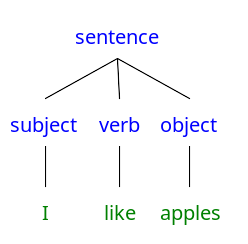
\includegraphics[width=5cm]{apple_tree.png}
 \caption{Parse tree}
  \label{parsetree}
\end{figure}
\end{example}


\subsection{Regular Grammar}
Let us now impose some restriction on the form of productions.

\begin{definition} 
A {\emph{regular grammar}} has $l \in NT $ and $ r = T$ or $T$ followed by $NT$.
\end{definition}

\begin{example}
The following is an example of a regular grammar:
\newline
N ::= 0 \newline
N ::= 1 \newline
N ::= 0N \newline
\end{example}

\end{document}
